\chapter{Design}
Now, once planed "What" is the system, it is needed to plan the "How" the system will be build in 
the implementation phase. Here is explained the components and the reason for it. As well
for the instructions on the system construction and realization.

\section{Analysis Review}

Taking in account the limited personal and time, some of what is specified in Analysis
has its scope reduced as to accomplish according to the requirements and constraints.
Using as inspiration the Copernicus SVP-BRST and the CMEMS labs previous experience,
the 5S can/ and will recall for used technology for easier design process.

The project then will be divided in three main parts; The Software, Hardware and the outer shell.
Then, lately, it will be shown the pieces of software used to accomplish this project. 

\section{Software}

As for software there will be two possible approaches for the problem, as the use of a RTOS
as stated on the Analysis, may require more time than it is worth. However, the use of a
RTOS, allow for a better control off timings and the low-power mode. Either way, as the
implementation of both alternatives may differ, the overall design will remain the same. 

This section will first decide the protocol available, abstractions, then the possibility of using a RTOS

\subsection{Communication protocol}

The selection of a network protocol is a complicated process as it interests with several
factors that imply directly on the data to be acquired. To list the ones with more influence.

\begin{itemize}
    \item Distance
    \item Bit-Rate
    \item Signal Availability (SIM card and protocol local integration)
    \item Price per package
    \item Integrated GNSS Hardware
    \item low-power
\end{itemize}

There are several protocols to choose from, so first it is needed to categorize the 
system needs and filter the list.

The first filter will be the distance. The IPC extends for kilometers along the shore, 
however signal along the shore can be mostly guaranteed as the service providers are 
mostly equally distributed. The real distinct characteristic is the reach offshore 
going inside the ocean. This category of protocol is a WWAN (Wireless Wide Area Network)

Some available protocols are; 2G(GS), 3G(UMTS), 4G(LTE), 5G, NB-IoT, Lora, Iridium

As the distance increases, the effective bit-rate tends to lower, due to protocols 
overhead and errors, so is espected a lower than usual bit-rate.

The protocol availability will depend on the service provider. This one is another set of
varieties itself, however it can be divided as local and global service providers. 

Services like SIMBASE, a global provider, are available for the lab to use, however it will offer coverage for 
a specific set of protocols in Portugal (coast). This one uses the local network interface,
so the coverage of each protocol depends on the local provider range of signal.

\begin{table}[h!]
    \centering
    \begin{tabular}{l|l|l|l|l|l|l}
        \textbf{Portugal} & \textbf{2G} & \textbf{3G} & \textbf{4G} & \textbf{5G} & \textbf{LTE-M} & \textbf{NB-IoT} \\
        \hline
        \arrayrulecolor[gray]{0.85}
        Meo      & V  & V  & V  & -- & -- & -- \\
        \hline
        Nos      & V  & V  & -- & -- & -- & -- \\
        \hline
        Vodafone & V  & -- & V  & V  & V  & -- \\
        \arrayrulecolor{black}
    \end{tabular}
    \caption{Protocol per provider table}
    \label{table:protocol_per_provider}
\end{table}


Doing a local search, the Vodafone service provider, differs from the others, as
also offers NB-IoT protocol if accorded directly.

By these factors, it is reducible to LTE and NB-IoT protocols. The price is inclined to
the LTE protocol, as is already available on lab, but the NB-IoT is more centered 
around the low-power. There are several boards that include both protocols with GNSS 
integrated so it also ain't a defining criterion.

As low-power is a main concern on this project, the NB-Iot is the chosen protocol, 
however the 4G is a strong alternative, in case of a substitution.
\subsection{Abstraction}

As the implementation require multiple communication protocols between components,
the development will require a layer of abstraction named wrappers. Protocols like OneWire, SPI and AT 
commands can and should be a higher level function, even with HAL assistance.

AT commands can be simplified to simpler functions without the necessity to write down
the command. As HAL handles the UART transmission by taking an array, it is possible to
use a sprintf to format the command using function parameters. Then it can be received 
the module answer and writing it on an array given when the function is called. 

As for the SPI, here the intention is to simplify the multiple registers needed to 
configure the system components like the IMU. A simple Get Function that sends a 
pre-defined signal, activating the right CS and making the communication easier.

The OneWire, as not covered by the HAL, can be the hardest one, as it would be needed
to be written from scratch. However, there is already libraries specific for the 
module in use, simplifying the process to program on this phase. 

%\subsection{RTOS}
%\subsection{RTOS alternative}

\section{Hardware}

This section elaborate on the system physical components, their connections and the 
reasons they were chosen. It is important to remember that the main objective, even if 
it is not specified on the topic, is the low-power functionalities. So the ability to
consume less power is a favoring point. 


\subsection{Autonomy}
Autonomy is the main point to look for as the system is designed, as the higher autonomy, 
the longer 5S can stay adrift without maintenance.

As for the autonomy there are two main factors to consider, the batteries and the board 
consumption To do it, so it is first need to set a consumption goal and the autonomy is 
good enough if the power needed is lower or equal then the goal.

Although the renewable energy is out of the scope of this project, the components suggested
for future improvements will be shown at the end as a possible future feature. 

As a restriction, the minimum amount of time in ocean is 1 month(720 hours), this will help us 
define the consumption goal.

\subsubsection{Board Consumption}
\label{link:Board Consumption}
Remembering the Analysis list of components, there are several components that consume
power in the system. And the sum of them will be used to choose the battery capacity.

The main power sinks in the systems will be the Microcontroller and the 
Communication Shield. As a head-start, choosing these two components will help. There are
several options for both, however it must be selected according to the settled rules. The
microcontroller has to be an STM32, containing the necessary peripheries, and the module have NB-IoT (And LTE just in case), both
with low-power functionalities.

According to the microcontroller rules, there are still several boards with the minimum
resources to accomplish the goal, even if it is selected the L0 models, designed for 
low-power. As this first prototype, it was selected a STM32H7, as it is available, 
that has an elevated power consumption, however it allows for a better system 
modulation. As the HAL is used, the transference for a future STML0 board model, 
with the necessary resources is mostly effortless. 

\begin{table}[h!]
    \centering
    \begin{tabular}{l|l|l}
        \textbf{Feature} & \textbf{STM32H7 $\mu$A/MHz} & \textbf{STM32L0 $\mu$A/MHz} \\ 
        \hline
        \arrayrulecolor[gray]{0.85}
        Run Current @ 3.3V & $\sim$600    & $\sim$87  \\
        \hline
        Sleep/Stop Mode    & $\sim$2.5    & $\sim$0.5 \\
        \hline
        Standby Mode       & $\sim$0.25   & $\sim$0.2 \\
        \hline
        Supply Voltage     & 1.62V to 3.6V & 1.65V to 3.6V \\
        \arrayrulecolor{black}
    \end{tabular}
    \caption{Typical power consumption values for STM32H7 vs STM32L0.}
    \label{table:typical_power_consumption_stm32}
\end{table}

Initial, the prototype will consume, on average as it will mostly stay on sleep mode
, 2.5 $\mu$A/MHz, and lately 0.5$\mu$A/MHz. 

As for he GNSS/NB-Iot or LTE module, there is several modules that fit the design rules.
The list of module available are SIM 7000,7020,7080,7600, Quectel BG77, Quectel BG95a 
and EVKITST87M01-1.

\begin{table}[h!]
    \centering
    \begin{tabular}{l|l|l|l}
        \textbf{Module} & \textbf{Sleep Mode (µA)} & \textbf{Idle Mode (mA)} & \textbf{Peak Current (mA)} \\
        \hline
        \arrayrulecolor[gray]{0.85}
        SIM7020         & 20    & N/A  & 2,000 \\
        \hline
        SIM7080G        & 600   & 10   & N/A   \\
        \hline
        SIM7000E        & 1,000 & 11   & 167   \\
        \hline
        SIM7600         & 2,800 & 18   & 896   \\
        \hline
        Quectel BG77    & 530   & 1    & 559.980 \\
        \hline
        Quectel BG95-M3 & 3,840 & 24   & 357   \\
        \hline
        EVKITST87M01-1  & N/A   & N/A  & N/A   \\
        \arrayrulecolor{black}
    \end{tabular}
    \caption{Current Consumption of Modules}
    \label{table:current_consumption_modules}
\end{table}

\begin{table}[h!]
    \centering
    \begin{tabular}{l|l|l|l|l|l}
        \textbf{Module} & \textbf{2G} & \textbf{3G} & \textbf{4G LTE} & \textbf{NB-IoT} & \textbf{GPS} \\
        \hline
        \arrayrulecolor[gray]{0.85}
        SIM7020         & No  & No  & No           & Yes & No  \\
        \hline
        SIM7080G        & No  & No  & No           & Yes & No  \\
        \hline
        SIM7000E        & Yes & No  & Yes          & Yes & Yes \\
        \hline
        SIM7600         & Yes & Yes & CAT4         & No  & Yes \\
        \hline
        Quectel BG77    & No  & No  & No           & Yes & Yes \\
        \hline
        Quectel BG95-M3 & Yes & No  & LTE-M/NB-IoT & Yes & Yes \\
        \hline
        EVKITST87M01-1  & No  & No  & No           & Yes & No  \\
        \arrayrulecolor{black}
    \end{tabular}
    \caption{Supported Protocols by Module}
    \label{table:supported_protocols_by_module}
\end{table}
 
In conclusion, the Module to choose is the SIM7000E, as it has the better 
average consume and has both protocols at disposal.

The following items were chosen by the laboratory availability.
\\\\
\textbf{IMU 9DOF GY-85 - ITG3205 + ADXL345 + HMC5883L}
\\\\
The \textbf{GY-85} is a compact Inertial Measurement Unit (IMU) that integrates three key motion sensors, offering 9 degrees of freedom (9DOF). It combines the following components:

\begin{itemize}
    \item \textbf{ITG-3205}: a 3-axis gyroscope for measuring angular velocity,
    \item \textbf{ADXL345}: a 3-axis accelerometer for detecting linear acceleration,
    \item \textbf{HMC5883L}: a 3-axis magnetometer for sensing magnetic fields and orientation.
    \item \textbf{Amperage consume}: 23uA while turned on.
\end{itemize}

Together, these sensors provide comprehensive motion and orientation data, 
making the GY-85 suitable for applications in robotics, drones, wearable 
devices, and general motion tracking systems. The module communicates using 
the I2C protocol, enabling easy integration with microcontrollers and 
embedded systems.

\begin{figure}[H]
    \centering
    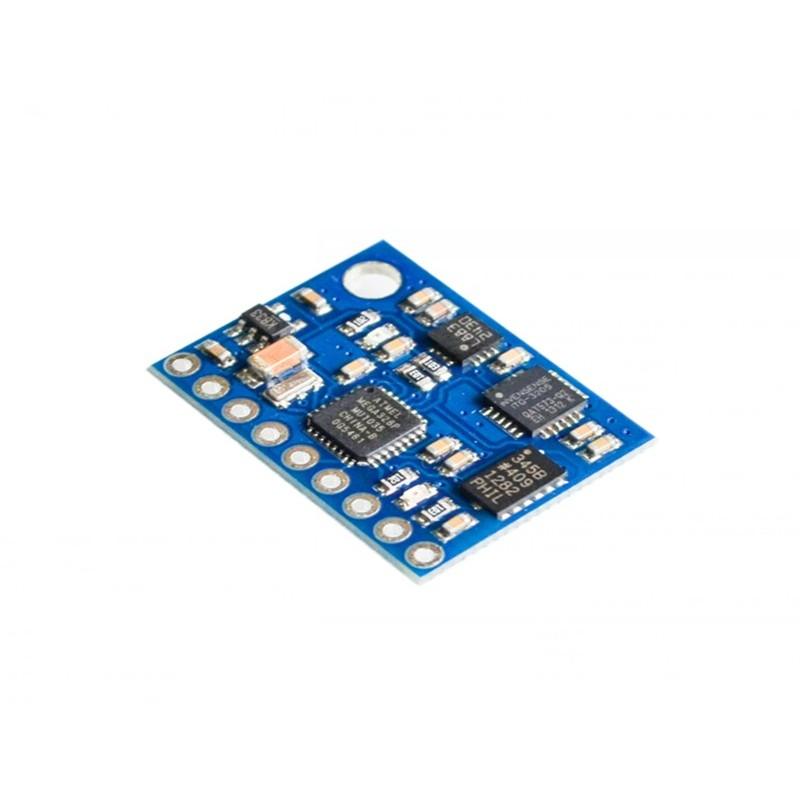
\includegraphics[width=0.35\textwidth]{images/chapter/design/components/final_IMU.png}  % Adjust the width as necessary
    \caption{9DOF GY-85 - ITG3205 + ADXL345 + HMC5883L}
    \label{fig:9DOF GY-85 - ITG3205 + ADXL345 + HMC5883L}        
\end{figure}

Taking an average consume of 23uA and speculating a 10\% usage over the whole cycle.

\( 23uA * 10\% = 2.3uA/Cicle\)

\textbf{SIM7000E Arduino NB-IoT/LTE/GPRS/GPS Expansion Shield}
\\\\
The \textbf{SIM7000E Expansion Shield} is a versatile communication module designed for use with Arduino boards. It integrates the \textbf{SIM7000E} cellular module, enabling support for multiple communication technologies, including:

\begin{itemize}
    \item \textbf{NB-IoT (Narrowband IoT)} for low-power, wide-area communication,
    \item \textbf{LTE Cat-M1} for efficient, low-latency data transmission,
    \item \textbf{GPRS/EDGE} as a fallback for 2G networks,
    \item \textbf{GPS} for accurate positioning and navigation.
    \item \textbf{Amperage consume} of 1 mA as it requests for data transference.
\end{itemize}

The shield is ideal for IoT applications requiring reliable connectivity and 
geolocation, such as asset tracking, environmental monitoring, smart 
agriculture, and remote sensing. It interfaces easily with Arduino via UART, 
making it accessible for both prototyping and deployment in embedded systems.

\begin{figure}[H]
    \centering
    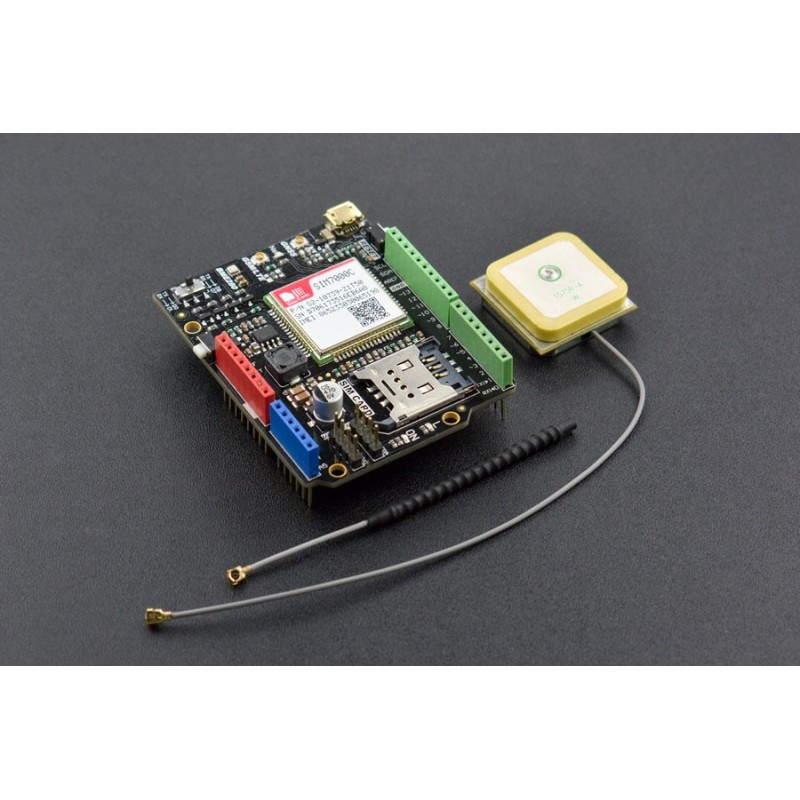
\includegraphics[width=0.7\textwidth]{images/chapter/design/components/SIM7000.png}  % Adjust the width as necessary
    \caption{SIM7000E}
    \label{fig:SIM7000E}        
\end{figure}

Using both LTE and GNSS and a usual assuming that would take around 1 minute to transmit, with 10 minutes cycle
,gives the systems a 10\% active mode per cycle as it. 

In Idle mode consumes 11mA, as in LTE and GNSS pulls for 167mA for both.

\( 11 mA×90\%+167 mA×10\%=9.9 mA+16.7 mA=26.6 mA/Cicle\)


\textbf{Waterproof Temperature Sensor (DS18B20)}\\\\
The \textbf{DS18B20} is a digital temperature sensor known for its accuracy, reliability, and ease of use. Encapsulated in a waterproof stainless steel probe, this version of the sensor is ideal for use in wet or outdoor environments.

Key features include:

\begin{itemize}
    \item \textbf{Temperature range}: -55°C to +125°C,
    \item \textbf{Accuracy}: ±0.5°C in the -10°C to +85°C range,
    \item \textbf{Digital output} via the \textbf{1-Wire} protocol, allowing multiple sensors to share a single data line,
    \item \textbf{Waterproof design} for robust operation in harsh environments.
    \item \textbf{Amperage consume} of 1mA per conversion.
\end{itemize} 

The DS18B20 is commonly used in applications such as HVAC systems, weather
stations, industrial temperature monitoring, and smart farming. Its simple 
interface and compatibility with microcontrollers like Arduino and STM32 
make it a popular choice for both hobbyist and professional projects.

\begin{figure}[H]
    \centering
    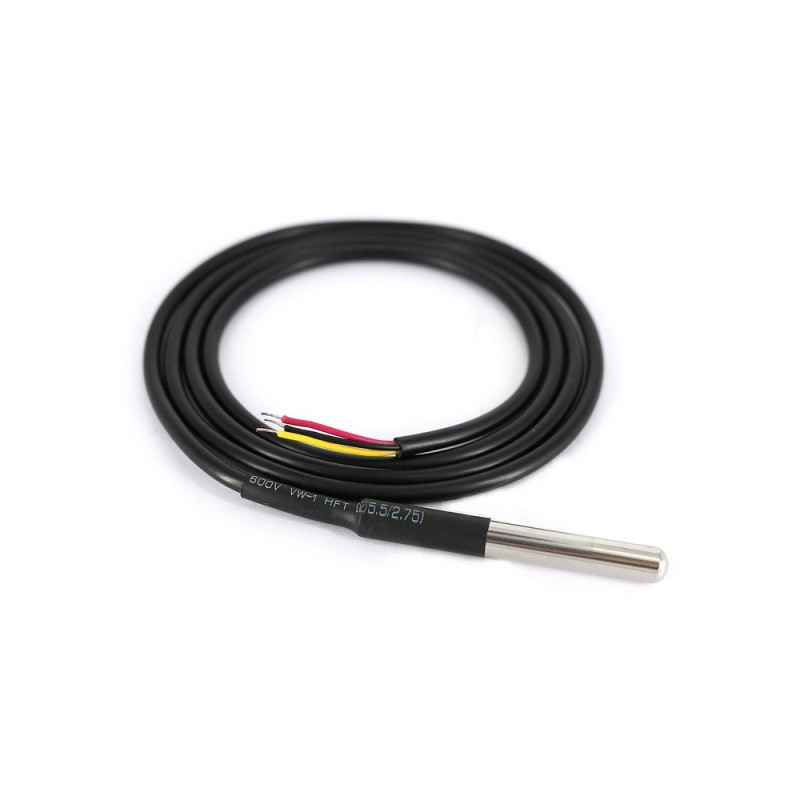
\includegraphics[width=0.5\textwidth]{images/chapter/design/components/temp.png}  % Adjust the width as necessary
    \caption{DS18B20}
    \label{fig:DS18B20}        
\end{figure}

Using the same formula as before, now with a 0.17\% as the module takes around 1 second per cycle, consuming 1mA

\(1mA*0.17\% = 0.0017mA = 1.7\mu A/Cicle \)

\textbf{Micro SDHC Card INF01016}\\\\
The size  of the SD card, will depend on the amount of data to be stored.
\\\\
\( Storage Size = \frac{Packege Size(bytes) * frac Time Online(H)}{Sample period(H)}\)
\\\\
Speculating that 5S will produce around 200 bytes each 10 minutes over 4 months
it is possible to reach the value of 
\\\\
\( Storage Size = \frac{200 * 4 * 30 * 24}{\frac{10}{60}} = 3.4Gbytes\)
%saize dimention
%sdcard.png

\begin{figure}[H]
    \centering
    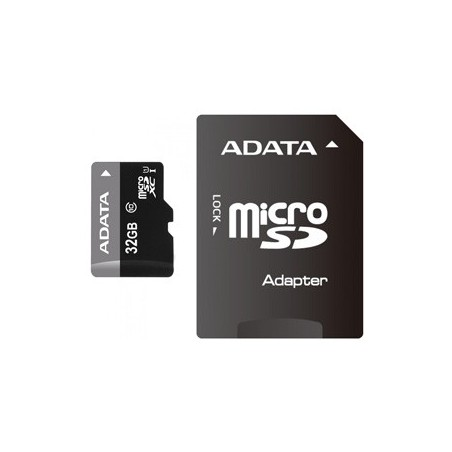
\includegraphics[width=0.45\textwidth]{images/chapter/design/components/sdcard.png}  % Adjust the width as necessary
    \caption{Micro SD card}
    \label{fig:Micro SD card}        
\end{figure}

At last, using the same values as the temperature sensor, the micro SD card will consume proximally the same.

\(1mA*0.17\% = 0.0017mA = 1.7 \mu A/Cicle \)

\textbf{Micro SDHC Card Reader Module and Battery Holder}\\\\
As the last components, there's will be used some support modules and battery 
support to hold the electronics in place.

\begin{figure}[H]
    \centering
    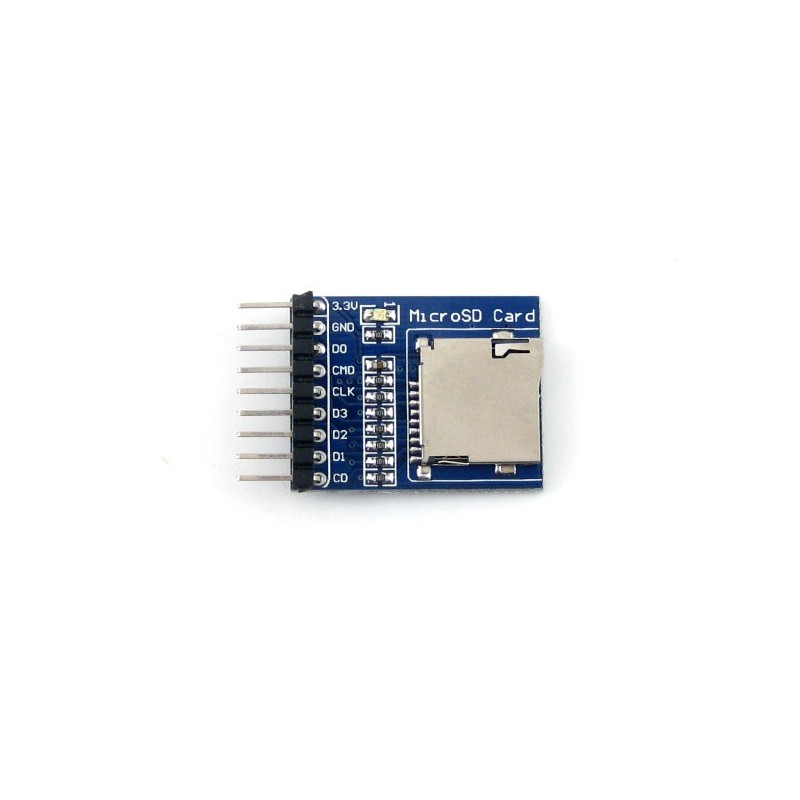
\includegraphics[width=0.3\textwidth]{images/chapter/design/components/sd_support.jpg}  % Adjust the width as necessary
    %\caption{Módulo leitor de cartões micro SD}
    \label{fig:Módulo leitor de cartões micro SD}        
    \hspace{0.1cm}
    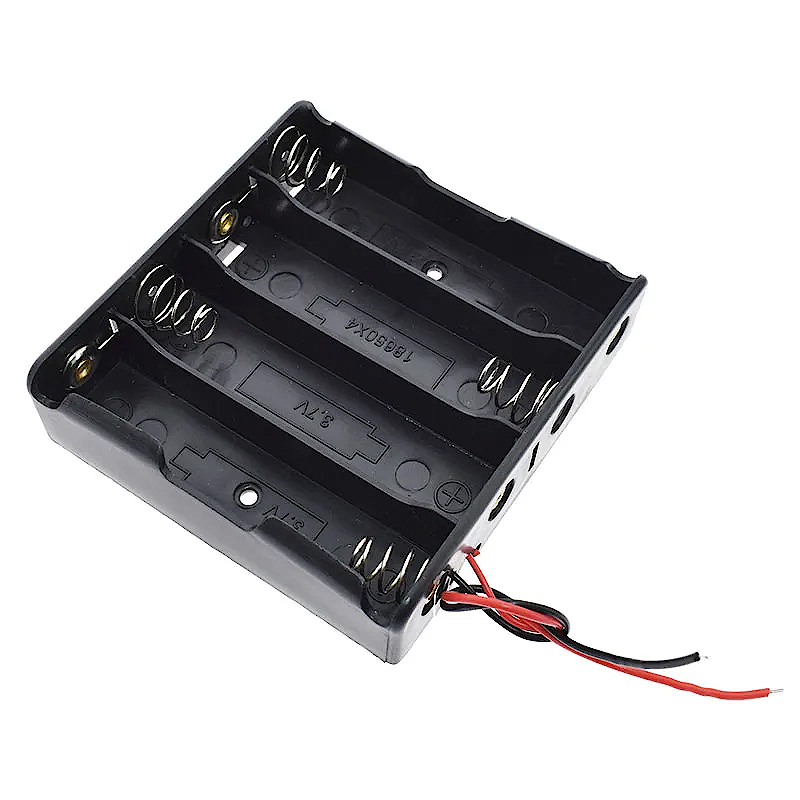
\includegraphics[width=0.2\textwidth]{images/chapter/design/components/battery-holder.jpg}  % Adjust the width as necessary
    \caption{Battery Holder}
    \label{fig:Battery Holder}        
\end{figure}




\subsubsection{Possible Solar Energy}
As an additional topic, here will be briefly explored the option of renewable
energy, for future exploration.

The module AEM10941 and the solar panel SM111K06L are good recommendations.Is ad
visible to follow the datasheet as the module requires specific configuration and circuits 
to work properly.

%\subsection{SDCard}
%\subsection{STM32}

%STM32L010K4T6
%microcontroler
%ADC
%UART
%SPI
%ONEWire
%\subsection{BMI088 IMU Sensor}
%gyroscope and acelerometer


%\subsection{Temperature}
%DS18B20



\subsubsection{Batteries}

Using the formula \( Battery Capacity = Amperage * Time\), it can be determinate the 
Amperage consumption limit. As Batteries capacity has a discrete value available on market,
it is possible to make a table as graph the results for better visualization.

Using the 3,7V batteries available by the laboratory, the following table can be constructed. 
\begin{table}[h!]
    \centering
    \begin{tabular}{l|l|l}
        \textbf{Cell Capacity (mAh)} & \textbf{Max Amperage (A)} & \textbf{Price (€)} \\
        \hline
        \arrayrulecolor[gray]{0.85}
        800  & 1.11 & 4.95 \\
        \hline
        2000 & 2.77 & 3.40 \\
        \hline
        2200 & 3.05 & 3.90 \\
        \hline
        2500 & 3.47 & 4.40 \\
        \hline
        2600 & 3.61 & 4.60 \\
        \hline
        3200 & 4.44 & 5.40 \\
        \hline
        3350 & 4.65 & 9.40 \\
        \arrayrulecolor{black}
    \end{tabular}
    \caption{Battery Capacities, Prices, and Current Capabilities}
    \label{table:battery_capacities}
\end{table}

However, 1 month is a short amount of time when the IPC cycle take almost one third of 
the year. Then, using more batteries, 5S will accomplish to acquire date of a full cycle.
As the equation for the Amperage consumption is linear, multiplying the amount of time by 
four implies four times the capacity meaning the system will support. Using the following table
the amount of current needed per cycle is estimated. 
\begin{table}[h!]
    \centering
    \begin{tabular}{l|l}
        \textbf{Component} & \textbf{Average Consumption} \\
        \hline
        \arrayrulecolor[gray]{0.85}
        STM32H7      & 27.25\,$\mu$A \\
        \hline
        SIM7000E     & 26.6\,mA \\
        \hline
        DS18B20      & 1.7\,$\mu$A \\
        \hline
        IMU (GY-85)  & 2.3\,$\mu$A \\
        \hline
        MicroSD Card & 1.7\,$\mu$A \\
        \hline
        \textbf{Total Estimated} & \textbf{26.63\,mA} \\
        \arrayrulecolor{black}
    \end{tabular}
    \caption{Average Power Consumption Per Component Per 10 Minutes Cicle}
    \label{table:average_consumption}
\end{table}

With a total of 26.63mA per cycle (mostly from the GNSS and LTE module), a system would need a 76Ah
capacity making 22 from the most expensive batteries. That is unreal and unpractical. Here would perfectly
fit a renewable source of energy such as solar or even harvest the wave undulation, however this is out of the
project scope. Making the project unable to fulfill the four months period all by himself, needing a change of 
batteries i between. So in order to make the least trips along these 4 months as possible. In order to do it,
was stipulated that 4 batteries was a good number, considering that it won't add as much weight. Then 
,in order to get the drifter autonomy, the value is divided by the system consumption. 

\begin{table}[H]
    \centering
    \small
    \setlength{\tabcolsep}{6pt}
    \begin{tabular}{l|l|l|l|l}
        \textbf{Total Ca\-pa\-ci\-ty} & \textbf{Total Price} & \textbf{Au\-to\-no\-my} & \textbf{Au\-to\-no\-my} & \textbf{Trips per Month} \\
        \textbf{(mAh)} & \textbf{(€)} & \textbf{(h)} & \textbf{(days)} & \\
        \hline
        \arrayrulecolor[gray]{0.85}
        3200  & 19.80 & 120.16 & 5.01  & 6 \\
        \hline
        8000  & 13.60 & 300.41 & 12.52 & 3 \\
        \hline
        8800  & 15.60 & 330.45 & 13.77 & 3 \\
        \hline
        10000 & 17.60 & 375.55 & 15.65 & 2 \\
        \hline
        10400 & 18.40 & 390.57 & 16.27 & 2 \\
        \hline
        12800 & 21.60 & 480.70 & 20.03 & 2 \\
        \hline
        13400 & 37.60 & 503.10 & 20.96 & 2 \\
        \arrayrulecolor{black}
    \end{tabular}
    \caption{Battery Capacity, Price, Estimated Autonomy, and Required Battery Swaps per Month}
    \label{table:battery_autonomy_trips}
\end{table}

So in order to make the least trips per month and pay less, four of the 2500mAh batteries are the ideal. 


%batt.jpg

\begin{figure}[H]
    \centering
    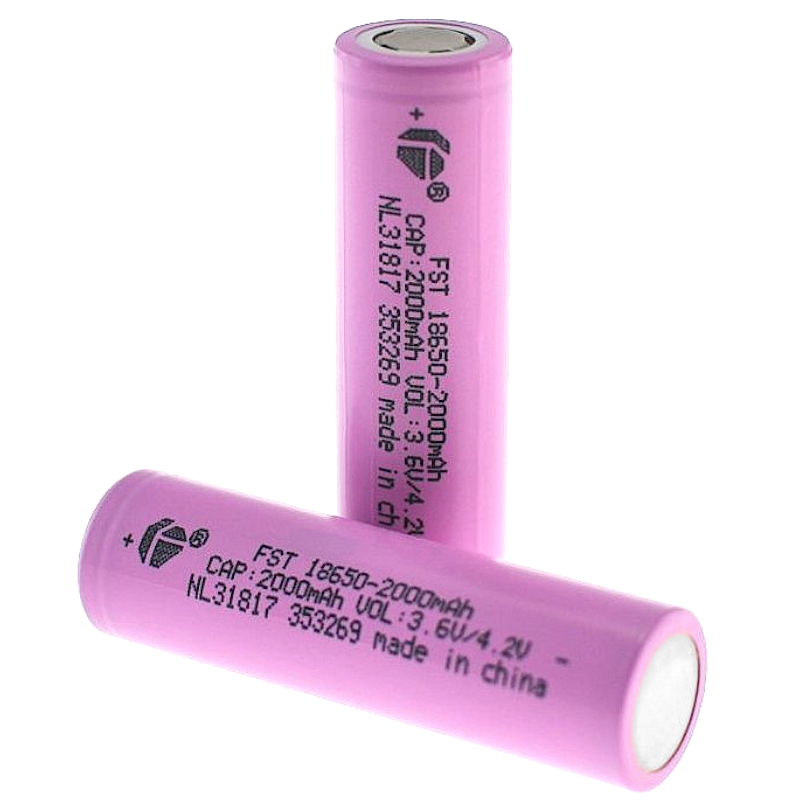
\includegraphics[width=0.3\textwidth]{images/chapter/design/components/batt.jpg}  % Adjust the width as necessary
    \caption{LI-ION 18650 3,7V 2000MAH}
    \label{fig:Battery}        
\end{figure}

\subsection{System Pinout}

Here will be displayed the systems' pinout. This table is used for further software and hardware development.

\begin{table}[h!]
    \centering
    \small
    \begin{tabular}{l|l|l}
        \textbf{Name} & \textbf{Pinout} & \textbf{uC Pin} \\
        \hline
        \arrayrulecolor[gray]{0.85}
        Temperature Sensor & VDD & 3.3V \\
         & GND & GND \\
         & Signal & PA0 (ADC1\_INP16) \\
        \hline
        IMU & VDD & 3.3V \\
         & GND & GND \\
         & SDA/SCL & PB9 / PB8 (I2C1) \\
        \hline
        UART AT & TX/RX & PA9 / PA10 (USART1) \\
        \hline
        UART DEBUG & TX/RX & PC10 / PC11 (USART3) \\
        \hline
        ADC Input & Signal & PA1 (ADC1\_INP17) \\
        \hline
        SD Card & VDD & 3.3V \\
         & GND & GND \\
         & CMD & PD2 (SDMMC1\_CMD) \\
         & CLK & PC12 (SDMMC1\_CK) \\
         & D0 & PC8 (SDMMC1\_D0) \\
         & D1 & PC9 (SDMMC1\_D1) \\
         & D2 & PC10 (SDMMC1\_D2) \\
         & D3 & PC11 (SDMMC1\_D3) \\
        \arrayrulecolor{black}
    \end{tabular}
    \caption{Peripheral Pinout Mapping to Microcontroller (STM32H755ZI-Q)}
    \label{table:peripheral_pinout}
\end{table}
\section{Shell}

Taking inspiration the SONDA drifter, the drifter's shell should have a way to conduct the wiring to the 
antennas and the temperature sensor and a basket to hold the electronics. Other point is to coat the 
electronics in plastic to waterproof the system.

The Shell has the following demands, as stated in analysis.

\begin{itemize}
    \item 2.5 dB Antenna should be at least 15 cm form water.
    \item The buoy should lift at least 500g ballast to hold the weight of the electronics and the pillars.
    \item The basket should have 10cm in diameter by 4cm in hight.
    \item It should be impact resistant to resist the waves and possible boat impacts.
\end{itemize} 

Using the Archmedes principle, to hold 500g of electronics on a 10cm in diameter by 4cm in hight it would
sink in water. So in order to float neutral of even float more secure, it would be necessary to project a 
buoy with the density according to the formula

\begin{equation}
    \rho_{\text{buoy}} = \frac{1000 \cdot (0.000314 + V_{\text{buoy}}) - 0.5}{V_{\text{buoy}}}
\end{equation}

Which, considering a 20cm per 4cm buoy it would make at least 
\(852 \, \text{kg/m}^3\) or lower.


\section{Tools and COTS}
\subsection{Tools}
\subsubsection{Inkscape}
A free and open-source vector graphics editor used for creating and editing SVG-based diagrams, schematics, and illustrations. Useful for generating custom graphics, PCB artwork, and documentation visuals.
\subsubsection{draw.io}
A web-based diagramming tool for creating flowcharts, system architectures, block diagrams, and wiring schematics. Supports real-time collaboration and integrates with cloud services like Google Drive and GitHub.
\subsubsection{STM32 CUBEmx}
A configuration and code generation tool for STM32 microcontrollers. Simplifies peripheral setup, clock tree configuration, and generates initialization C code for use with IDEs like STM32CubeIDE or Keil.
\subsubsection{Fusion360}
A professional-grade 3D CAD, CAM, and CAE tool from Autodesk. Used for mechanical design, simulation, and 3D modeling, making it ideal for designing enclosures, mounts, and mechanical parts.
\subsubsection{\LaTeX}
A high-quality typesetting system used for technical and scientific documentation. Ideal for creating well-formatted reports, theses, datasheets, and documentation with complex mathematical content
\subsubsection{Minicom}
Minicom is a text-based serial communication program for Unix-like systems. It allows you to connect to serial devices (like routers, microcontrollers, or modems) via a serial port (e.g., /dev/ttyACM0). It's commonly used for debugging, configuration, and monitoring of hardware over UART.
\subsection{COTS}
All COTS are specified on the \hyperref[link:Board Consumption]{Board Consumption} chapter.
%\section{Theorical Concepts}